\apendice{Documentación}

\section{Requisitos software y hardware para ejecutar el proyecto}
Todo esto se encuentra en la referencia \cite{mathworks_system_requirements_matlab}.
\subsection{Requisitos de software}
Sistema operativo compatible: Windows 10 (64 bits) o superior. También compatible con macOS Mojave o superior y algunas distribuciones Linux (Ubuntu 18.04+)

Entorno principal de desarrollo:
MATLAB R2019b (versión 9.7.0, actualización 9 – Build 1737446). Fecha de instalación usada en este proyecto: 5 de agosto de 2021

Toolboxes de MATLAB requeridos:
\begin{itemize}
    \item Simulink: para diseño y simulación visual de sistemas dinámicos.
    \item Control System Toolbox: para diseñar y ajustar el regulador PID.
    \item App Designer: entorno visual para crear la interfaz de usuario (GUI).
\end{itemize}

Todas las herramientas fueron utilizadas bajo licencia académica, válida para investigación y docencia.

\subsection{Requisitos hardware}
En la tabla \ref{tab:requisitos}\footnote{las simulaciones complejas en Simulink con controladores PID y grandes datos pueden requerir mayor capacidad de RAM.} se encuentran los requisitos mínimos y recomendados para el hardware.

\begin{table}[H]
\small
\centering
\resizebox{\textwidth}{!}{%
\begin{tabular}{|l|c|c|}
\hline
\textbf{Recurso}         & \textbf{Mínimo}                      & \textbf{Recomendado}                    \\
\hline
Procesador               & Intel Core i3 / AMD Ryzen 3          & Intel Core i5 o superior                \\
\hline
Memoria RAM              & 4 GB                                 & 8--16 GB (para simulaciones en Simulink) \\
\hline
Espacio en disco         & 2 GB libres                          & 5 GB (con resultados y backups)         \\
\hline
GPU (opcional)           & No requerida                         & Compatible con OpenGL                   \\
\hline
Resolución de pantalla   & 1366$\times$768                      & 1920$\times$1080                        \\
\hline
\end{tabular}
} % Fin del resizebox
\caption{Requisitos mínimos y recomendados para la ejecución del proyecto.}
\label{tab:requisitos}
\end{table}



\section{Instalación / Puesta en marcha}
Este apartado explica cómo instalar el software necesario y cómo ejecutar la aplicación y simulaciones desarrolladas.

\subsection{Instalación de MATLAB}
Para la ejecución del proyecto es necesario disponer de una instalación funcional de MATLAB R2019b o superior. A continuación, se detallan los pasos básicos para su instalación con licencia académica:
\begin{enumerate}
    \item Acceder a la página oficial \cite{mathworks_matlab} y crear una cuenta usando el correo de la universidad.
    \item Tras iniciar sesión, buscar la opción "Get MATLAB" y seguir las instrucciones para asociar la cuenta a la licencia de la universidad, la UBU si dispone de ella. 
    \item Descargar el instalador correspondiente al sistema operativo (Windows, macOS o Linux).
    \item Ejecución del instalador. Iniciar sesión con la cuenta MathWorks y seleccionar la licencia asociada. Elegir los productos a instalar: MATLAB, Simulink, App Designer, Control System Toolbox, etc. Finalizar la instalación siguiendo las instrucciones del asistente.
    \item Abrir MATLAB desde el menú de inicio y comprobar su funcionamiento.
\end{enumerate}

\subsection{Ejecución del proyecto}
Una vez instalado MATLAB, se recomienda seguir los siguientes pasos para ejecutar correctamente el proyecto:
\begin{enumerate}
    \item Abrir MATLAB R2019b.
    \item Descargar o clonar el proyecto en una carpeta local.
    \item Añadir la carpeta raíz al path de MATLAB, como se ve en la imagen \ref{fig:instruccion}, escribir en la ventana de comandos
    \begin{figure}[H]
        \centering
        
\includegraphics[width=0.9\textwidth]{img/puesta en marcha.png}
        \caption{Instrucción de MATLAB para el paso 3.}
        \label{fig:instruccion}
        
    \end{figure}
    Cambiar 'ruta/del/proyecto' por la ruta en la que se tenga el proyecto.
    Sirve para añadir al path\footnote{Ruta de búsqueda, conjunto de carpetas donde MATLAB busca archivos cuando se ejecutan comandos o funciones.} de MATLAB la carpeta principal del proyecto y todas sus subcarpetas, de modo que MATLAB pueda acceder a todos los archivos, funciones, scripts y modelos sin errores. No hay que estar navegando carpeta por carpeta o copiando archivos manualmente.
    \item Para lanzar la aplicación con interfaz gráfica, abrir el archivo .mlapp desde o ejecutar en la ventana de comandos de MATLAB lo que se ve en la figura \ref{fig:app abrir}
    \begin{figure}[H]
        \centering
        
\includegraphics[width=0.9\textwidth]{img/abrir app.png}
        \caption{Instrucción de MATLAB para abrir la aplicación.}
        \label{fig:app abrir}
    \end{figure}
    \item Los modelos desarrollados en Simulink se encuentran organizados dentro de la carpeta Simulink/Modelos Simulink, con extensión .slx. Para abrir cualquiera de ellos, basta con hacer doble clic sobre el archivo correspondiente.
   
    Por otro lado, los scripts de MATLAB se localizan en la carpeta matlab y tienen extensión .m. Al igual que los modelos, estos pueden abrirse directamente haciendo doble clic sobre el archivo. 
    Una vez abiertos en el entorno, la ejecución se realiza pulsando el botón Run, que se puede observar en la figura \ref{fig:app run} donde se encuentra.

    \begin{figure}[H]
        \centering
        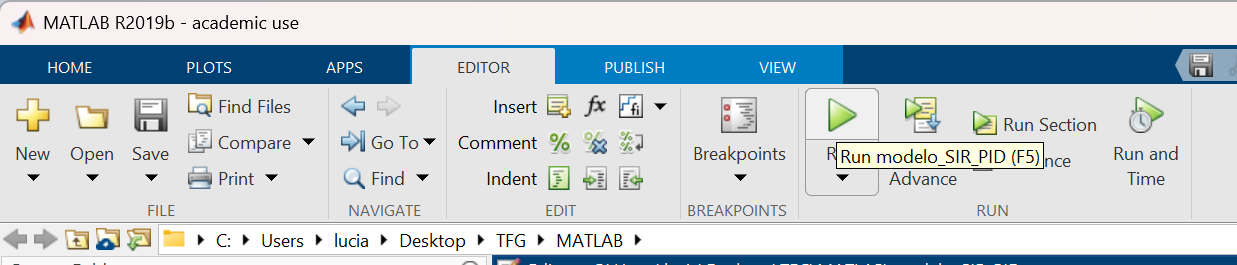
\includegraphics[width=0.9\textwidth]{img/run.png}
        \caption{Botón de Run de MATLAB.}
        \label{fig:app run}
        
    \end{figure}
\end{enumerate}



\section{Manuales y/o demostraciones prácticas}
\subsection{Interfaz principal de la aplicación}
La interfaz principal de la aplicación, desarrollada con App Designer de MATLAB, presenta un entorno intuitivo para simular diferentes modelos epidemiológicos. La pantalla inicial se muestra en la figura \ref{fig:app inicio}


\begin{figure}[H]
        \centering
        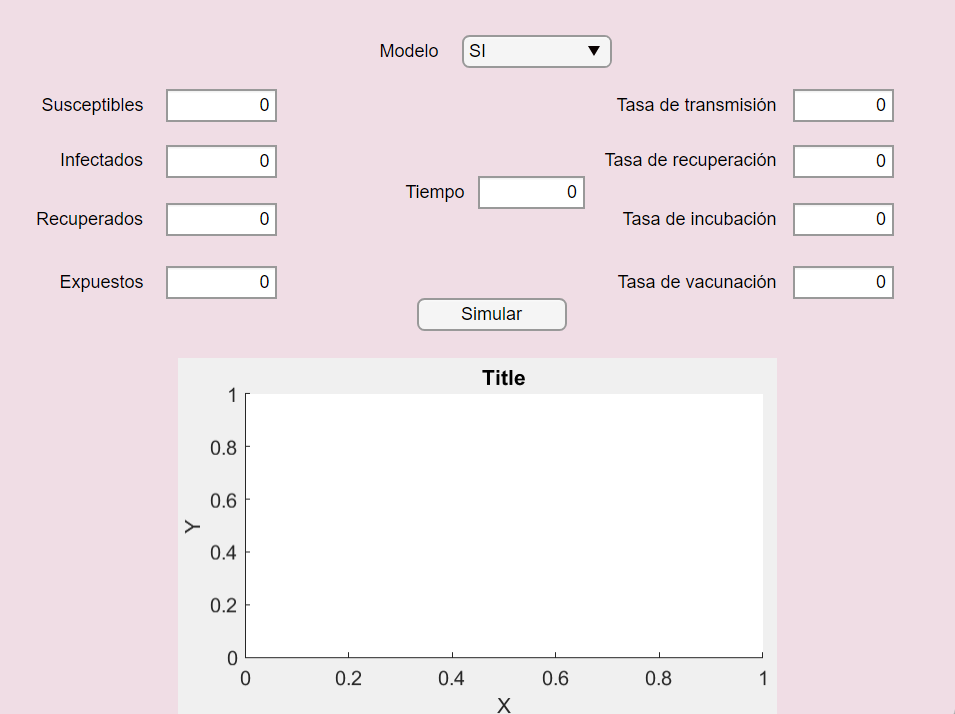
\includegraphics[width=0.9\textwidth]{img/inicio app.png}
        \caption{Interfaz inicial de la aplicación.}
        \label{fig:app inicio}
        
    \end{figure}

Desde el menú desplegable superior se puede seleccionar el modelo deseado entre SI, SIS, SIR, SEIR. A continuación, el usuario puede introducir los valores iniciales para cada grupo de población:
\begin{itemize}
    \item Susceptibles
    \item Infectados
    \item Recuperados
    \item Expuestos
\end{itemize}
Así como las tasas características del modelo:
\begin{itemize}
    \item Tasa de transmisión
    \item Tasa de recuperación
    \item Tasa de incubación
    \item Tasa de vacunación
\end{itemize}
También se introduce el tiempo de simulación total (en días o unidades temporales equivalentes). Una vez completados los parámetros, el botón "Simular" permite ejecutar la simulación. Los resultados se visualizan automáticamente en una gráfica situada en la parte inferior.

Esta interfaz facilita el análisis comparativo entre modelos y permite observar el comportamiento dinámico del sistema epidemiológico en función de las distintas condiciones iniciales.

\subsection{Selección del modelo}

La aplicación permite seleccionar el tipo de modelo epidemiológico a simular mediante un menú desplegable ubicado en la parte superior central de la interfaz. Los modelos disponibles son:

\begin{itemize}
    \item \textbf{SI}: modelo simple de contagio sin recuperación.
    \item \textbf{SIS}: permite reinfección tras la recuperación.
    \item \textbf{SIR}: incluye inmunidad permanente tras la recuperación.
    \item \textbf{SEIR}: añade una fase de exposición previa al contagio.
    \item \textbf{SIRV}: añade una tasa de vacunación al modelo SIR.
    \item \textbf{SEIRV}: añade tasa de vacunación al modelo SEIR.
\end{itemize}

Al seleccionar un modelo, la interfaz se adapta automáticamente, activando o desactivando los campos de entrada correspondientes. Por ejemplo, el campo “Expuestos” sólo se habilita si se selecciona el modelo SEIR, y la “Tasa de vacunación” se emplea únicamente en aquellos modelos que incorporan estrategias de vacunación como SIRV o SEIRV. Además al seleccionar un modelo, se cargan automáticamente valores por defecto en todos los parámetros y campos de entrada. Esto permite ejecutar simulaciones de ejemplo directamente, sin necesidad de introducir manualmente todos los datos. Estos valores predefinidos están pensados para ofrecer resultados representativos del comportamiento típico de cada modelo.


\subsection{Ejecución de simulaciones}

Una vez configurados los valores iniciales de la población y los parámetros del modelo, el usuario debe presionar el botón \textbf{Simular}. Al hacerlo, se ejecuta la resolución del sistema de ecuaciones diferenciales asociado al modelo epidemiológico. Las simulaciones se realizan empleando funciones de MATLAB basadas en ode45, y los resultados se visualizan directamente en el eje gráfico de la interfaz. Las curvas generadas permiten analizar el comportamiento de cada grupo poblacional en el tiempo.

El sistema también incluye controles para reiniciar los parámetros y ejecutar nuevas simulaciones con diferentes configuraciones.

\subsection{Casos de uso prácticos}

A continuación, se presentan dos ejemplos prácticos de uso de la aplicación, explicados paso a paso. Estos permiten comprobar cómo se comporta la simulación en diferentes escenarios epidemiológicos.

\vspace{1em}
\subsubsection{Ejemplo 1 – Simulación con modelo SIR}

\textbf{Pasos:}
\begin{enumerate}
    \item Seleccionar el modelo \textbf{SIR} en el menú desplegable \ref{fig:eleccion sir}.
    \begin{figure}[H]
        \centering
        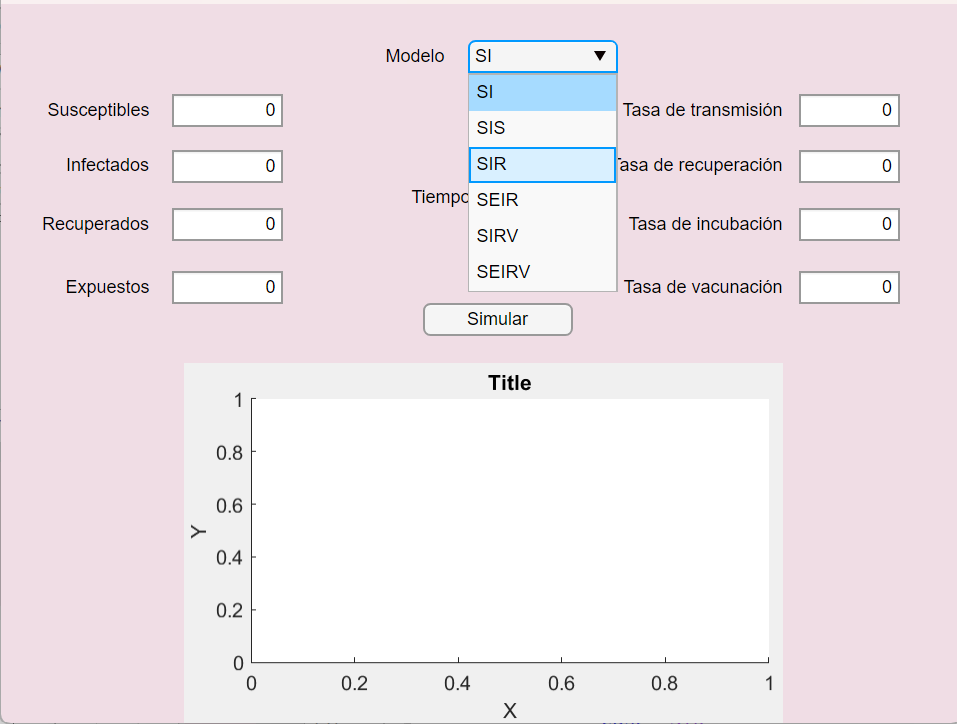
\includegraphics[width=0.9\textwidth]{img/eleccion modelo SIR.png}
        \caption{Elección del modelo, en este caso SIR.}
        \label{fig:eleccion sir}
        
    \end{figure}
    
     \item Verificar que los valores por defecto se han cargado correctamente (se pueden modificar si se desea)\ref{fig:datos defecto}.

\begin{figure}[H]
        \centering
        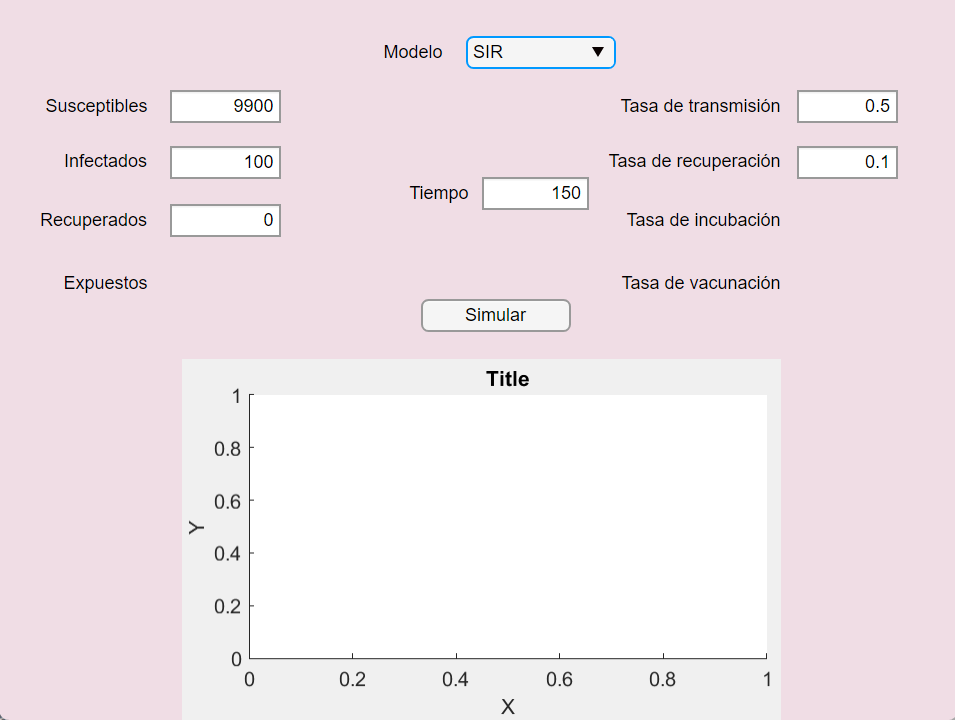
\includegraphics[width=0.9\textwidth]{img/modelo sir datos.png}
        \caption{Comprobación de que salen los datos por defecto.}
        \label{fig:datos defecto}
       
    \end{figure}
     
      \item Pulsar el botón \textbf{Simular}.

     
    \item Observar la evolución temporal de las tres poblaciones en la gráfica \ref{fig:simulacion sir ap}
    
   

    
   
   
    \begin{figure}[H]
        \centering
        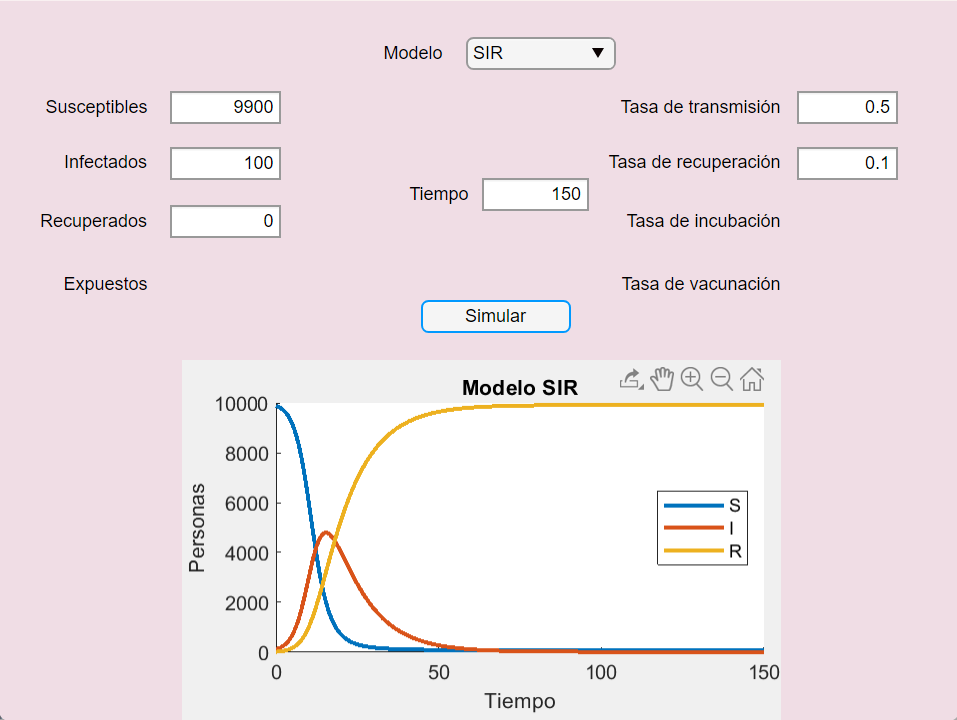
\includegraphics[width=0.9\textwidth]{img/simulacion sir app.png}
        \caption{Simulación del modelo SIR en la aplicación.}
        \label{fig:simulacion sir ap}
        
    \end{figure}
\end{enumerate}

Este ejemplo permite visualizar cómo aumenta inicialmente el número de infectados, hasta alcanzar un pico, seguido de una disminución conforme los individuos se recuperan y se inmunizan.

\vspace{1em}
\subsubsection{Ejemplo 2 – Simulación con modelo SEIR}

\textbf{Se siguien los mismos pasos que antes:}
\begin{enumerate}
    \item Seleccionar el modelo \textbf{SEIR} \ref{fig:eleccion seirv}.

    \begin{figure}[H]
        \centering
        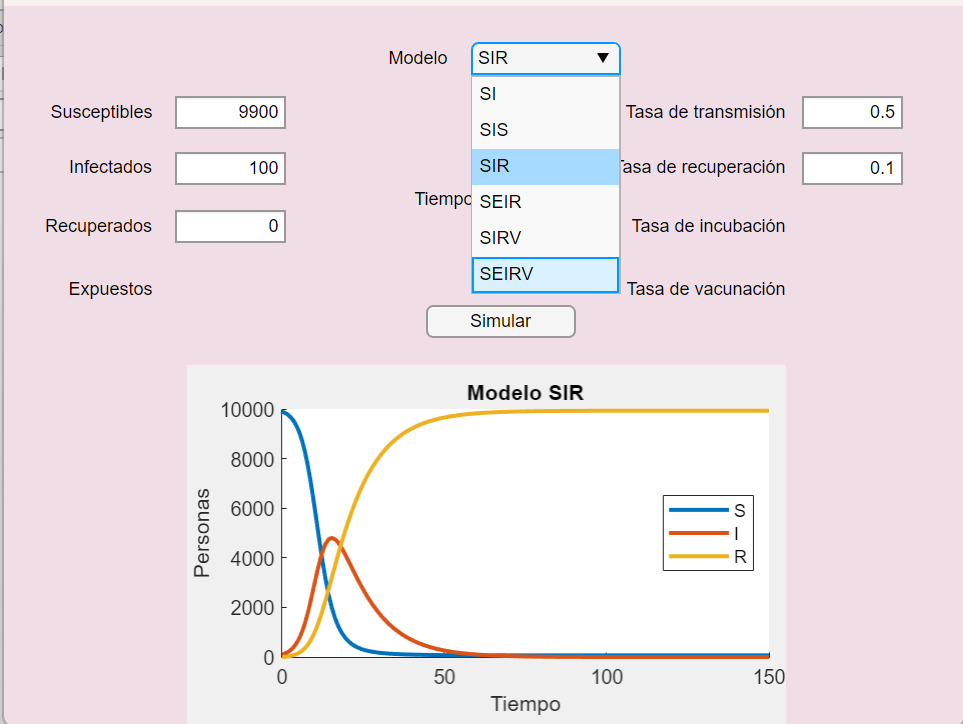
\includegraphics[width=0.9\textwidth]{img/eleccion SEIR.png}
        \caption{Elección del modelo, en este caso SEIRV.}
        \label{fig:eleccion seirv}
        
    \end{figure}
    \item Comprobar que los valores se han precargado automáticamente, se pueden cambiar si se desea.
    \item Hacer clic en \textbf{Simular}.
    \item Observar el efecto del regulador PID: el número de infectados se mantiene bajo control y disminuye más rápidamente \ref{fig:eseeir}.
\end{enumerate}




\begin{figure}[H]
        \centering
        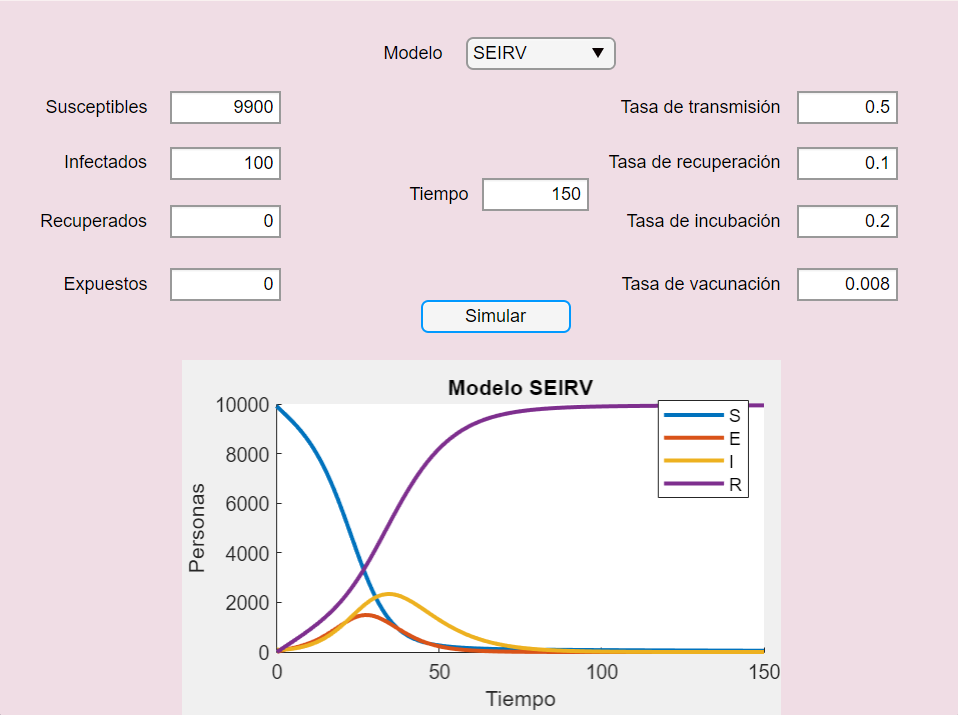
\includegraphics[width=0.9\textwidth]{img/simulacion.png}
        \caption{Simulación del modelo SEIRV en la aplicación con los datos predefinidos.}
        \label{fig:eseeir}
       
    \end{figure}









